\section*{ĐỀ TRẮC NGHIỆM CUỐI CHƯƠNG}
\Opensolutionfile{ans}[ans/ansTL-CD4]
\setcounter{ex}{0}
\subsubsection{Đề số 1}

\begin{ex}%[0D1Y4-1]
	Cho tập hợp $A=\left\{x \in \mathbb{R}|4 \leq x \leq 9\right\}.$ Sử dụng các kí hiệu ``khoảng'', ``nửa khoảng'' và ``đoạn'' để viết lại tập $A$.
	\choice
	{$A=(4;9]$}
	{\True $A=[4;9]$}
	{$A=[4;9)$}
	{$(4;9)$}
	\loigiai{
		Ta có $A=\left\{x \in \mathbb{R}|4 \leq x \leq 9\right\}$ nên
		$A=[4;9]$.}
\end{ex}

\begin{ex}%[0D1Y1-3]
	Tìm mệnh đề phủ định của mệnh đề sau \lq \lq $\forall x \in \mathbb{R},x^2 \geq 0$ \rq \rq.
	\choice
	{\lq \lq $\forall x \in \mathbb{R},x^2<0$ \rq \rq}
	{\lq \lq $\forall x \in \mathbb{R},x^2>0$ \rq \rq}
	{\True \lq \lq $\exists x \in \mathbb{R},x^2<0$ \rq \rq}
	{\lq \lq $\exists x \in \mathbb{R},x^2 \geq 0$ \rq \rq}
	\loigiai{
		Mệnh đề phủ định cần tìm là \lq \lq $\exists x \in \mathbb{R},x^2<0$ \rq \rq.}
\end{ex}

\begin{ex}%[0D1Y2-2]
	Cho tập hợp $M=\{1;2;3;4;5\}$. Số các tập con của $M$ luôn chứa cả ba phần tử $1$, $3$, $5$ là
	\choice
	{$3$}
	{$2$}
	{\True $4$}
	{$8$}
	\loigiai{
		Các tập con của $M$ luôn chứa cả ba phần tử $1$, $3$, $5$ là $\{1;3;5\}$, $\{1;3;5;2\}$, $\{1;3;5;4\}$, $\{1;3;5;2;4\}$.
	}
\end{ex}

\begin{ex}%[0D1Y1]
	Mệnh đề nào sau đây là đúng?
	\choice
	{\True $\exists n\in\mathbb{N}: n^2=n$}
	{$\forall n\in\mathbb{N}: n^2>0$}
	{$\forall n\in\mathbb{N}: n^2+1$ là số lẻ}
	{$\exists n\in\mathbb{N}: n^2-2=0$}
	\loigiai{
	Xét mệnh đề $\exists n\in\mathbb{N}: n^2=n$. Với $n=1$ thì $1^2=1$ nên đây là mệnh đề đúng.
	}
\end{ex}

\begin{ex}%[0D1B1]
	Trong các câu khẳng định sau, câu nào là mệnh đề \textbf{sai}?
	\choice
	{Tổng $3$ góc trong của một tam giác bằng $180^\circ$}
	{\True Nếu tam giác $ABC$ thỏa mãn $AB^2+AC^2=BC^2$ thì tam giác $ABC$ vuông tại $B$}
	{2 là số nguyên tố}
	{Nếu một phương trình bậc hai có biệt thức $\Delta$ không âm thì nó có nghiệm}
	\loigiai{
		Nếu tam giác $ABC$ thỏa mãn $AB^2+AC^2=BC^2$ thì tam giác $ABC$ vuông tại $A$ nên khẳng định tam giác vuông tại $B$ là sai.
	}
\end{ex}

\begin{ex}%[0D1B3]
	Cho hai tập hợp $A = \left\{ 0, 1, 2,  3, 4, 5 \right\}$ và $B = \left\{-2, 1, 4, 6\right \}$. Tìm tập hợp $A \setminus B$.
	\choice
	{\True $\left\{0, 2, 3, 5\right\}$}
	{ $\left\{0, 1, 2, 3, 4\right\}$}
	{$\left\{1, 4\right\} $}
	{$\left\{-2, 0, 1, 2, 3, 4, 5, 6\right\}$}
	\loigiai{
		Với $A \setminus B$ thì ta lấy những phần tử thuộc $A$ mà không thuộc $B$. Suy ra
		$$A \setminus B=\left\{0, 2, 3, 5\right\}.$$
	}
\end{ex}

\begin{ex}%[0D1B2-1]
	Hỏi tập hợp $A=\{k^2+1\mid k \in \mathbb{Z},|k| \leq 2\}$ có bao nhiêu phần tử?
	\choice
	{\True $3$}
	{$5$}
	{$2$}
	{$1$}
	\loigiai{
		Ta có $|k| \leq 2,k \in \mathbb{Z} \Leftrightarrow k \in \{\pm 1;0;\pm 2\}$.\\
		\begin{listEX}[2]
			\item [$\bullet$] Với $ k= \pm 2$, suy ra $k^2+1=5$.
			\item [$\bullet$] Với $ k= \pm 1$, suy ra $k^2+1=2$.
			\item [$\bullet$] Với $ k= 0$, suy ra $k^2+1=1$.
	\end{listEX}
Vậy, tập $A$ có 3 phần tử.}
\end{ex}


\begin{ex}%[0D1B1]
	Cho mệnh đề chứa biến $P(x):``x+15 \le x^2,\;x \in \mathbb{R}"$. Trong các mệnh đề sau, mệnh đề nào đúng?
	\choice
	{$P(3) $}
	{$P(4) $}
	{$P(0) $}
	{\True $P(5) $}
	\loigiai{
	Thử trực tiếp các giá trị của biến
	\begin{listEX}[2]
			\item [$\bullet$] Với $x=3$ thì $3+15 \le 3^2$ (sai).
		\item [$\bullet$] Với $x=4$ thì $4+15 \le 4^2$ (sai).
		\item [$\bullet$] Với $x=0$ thì $0+15 \le 0^2$ (sai).
		\item [$\bullet$] Với $x=5$ thì $5+15 \le 5^2$ (đúng).
	\end{listEX}
Suy ra $P(5)$ đúng.
	}
\end{ex}

\begin{ex}%[0D1B3-2]
	Tập hợp nào sau đây chỉ gồm các số vô tỷ?
	\choice
	{\True $\mathbb{R} \setminus \mathbb{Q}$}
	{$\mathbb{Q} \setminus \mathbb{N}^*$}
	{$\mathbb{Q} \setminus \mathbb{Z}$}
	{$\mathbb{R} \setminus \{0\}$}
	\loigiai{
		Ta có $\mathbb{R} \setminus \mathbb{Q}=I$ là tập hợp các số vô tỷ.}
\end{ex}

\begin{ex}%[0D1B4-1]
	Tập hợp $(-\infty;2] \cap (-6;+\infty)$ bằng tập nào dưới đây?
	\choice
	{\True $(-6;2]$}
	{$(-\infty;+\infty)$}
	{$[-6;2]$}
	{$(-6;2)$}
	\loigiai{
		Ta có $(-\infty;2] \cap (-6;+\infty)=(-6;2]$.
	}
\end{ex}

\begin{ex}%[0D1B3]
	Cho hai tập hợp $A=\left\{x\big| x\in\mathbb{R}\right\}$ và $B=(0;+\infty)$. Tìm tập hợp $A\setminus B$.
	\choice
	{$(0;+\infty)$}
	{$(-\infty;0)$}
	{$[0;+\infty)$}
	{\True $(-\infty;0]$}
	\loigiai{
	}
\end{ex}

\begin{ex}%[0D1B2]
	Tập hợp $A=\left\{x\in \mathbb{R}\big| 0<x<2 \right\}$ bằng tập hợp nào dưới đây?
	\choice
	{$[0; 2]$}
	{$\left\{0; 2\right\}$}
	{$(0; 2]$}
	{\True $(0; 2)$}
	\loigiai{
	}
\end{ex}

\begin{ex}%[Vũ Công Hoan]%[0D1Y4-1]%
	Hình vẽ dưới đây (phần không bị gạch chéo) biểu diễn cho tập hợp nào?
	\begin{center}
		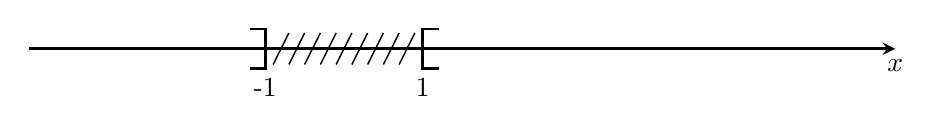
\begin{tikzpicture}[>=stealth]
			\def\gachtr[#1](#2){
				\path[#1, line width=0.5pt](#2-0.1,-0.2)--(#2+0.1,0.2);}
			\def\gachph[#1](#2){
				\path[#1, line width=0.5pt](#2-0.1,0.2)--(#2+0.1,-0.2);}
			\def\ngvmo[#1](#2){
				\path[#1, line width=1pt](#2+0.2,0.25)--(#2,0.25) -- (#2,-0.25)node[below]{#2}--(#2+0.2,-0.25);}
			\def\ngvdong[#1](#2){
				\path[#1, line width=1pt](#2-0.2,0.25)--(#2,0.25) -- (#2,-0.25)node[below]{#2}--(#2-0.2,-0.25);}
			\draw[->, line width=1pt] (-4,0) --(7,0)node[below]{$x$};
			\foreach \x in {-0.8,-0.6,...,0.8}{\gachtr[draw](\x)}
			\ngvmo[draw](1)
			\ngvdong[draw](-1)
		\end{tikzpicture}
	\end{center}
	\choice
	{$(-\infty;1)$}
	{$A=[-1;1]$}
	{\True$(-\infty;-1] \cup [1;+\infty)$}
	{$(1;+\infty)$}
	\loigiai{
		Phần không bị gạch chéo biểu diễn tập hợp $(-\infty;-1] \cup [1;+\infty)$.
	}
\end{ex}

\begin{ex}%[0D1B1-2]
	Trong các mệnh đề sau, mệnh đề nào \textbf{sai}?
	\choice
	{Nếu hai tam giác bằng nhau thì hai tam giác đó đồng dạng}
	{Nếu hai tam giác bằng nhau thì bán kính đường tròn ngoại tiếp của hai tam giác đó bằng nhau}
	{Nếu hai tam giác bằng nhau thì hai tam giác đó diện tích bằng nhau}
	{\True Nếu hai tam giác có bán kính đường tròn ngoại tiếp bằng nhau thì hai tam giác đó bằng nhau}
	\loigiai{
		Có thể lấy ví dụ về hai tam giác vuông cùng có cạnh huyền bằng $a$ nhưng các cạnh góc vuông không bằng nhau, suy ra nhận xét Nếu hai tam giác có bán kính đường tròn ngoại tiếp bằng nhau thì hai tam giác đó bằng nhau là sai.}
\end{ex}

\begin{ex}%[0D1B3-1]
	Cho tập hợp $X=(-\infty;2] \cap (-6;+\infty)$. Khẳng định nào sau đây là đúng?
	\choice
	{\True $X=(-6;2]$}
	{$X=(-\infty;+\infty)$}
	{$(-6;+\infty)$}
	{$X=(-\infty;2]$}
	\loigiai{
		Ta có: $X=(-\infty;2] \cap (-6;+\infty)=(-6;2]$.}
\end{ex}

\begin{ex}%[0D1B4]
	Cho các tập hợp $A=(-2;15)$ và  $B=(3;+ \infty )$. Khi đó $A \cup B$ là tập hợp nào sau đây?
	\choice
	{$[15;+\infty ) $}
	{$(-2;3] $}
	{\True $(-2;+ \infty ) $}
	{$(3;15) $}
	\loigiai{
	}
\end{ex}

\begin{ex}%[0D1B2]
	Hãy viết tập hợp $A=\left\{x\in \mathbb{R}\big| 2x^2-3x+1=0\right\}$ dưới dạng liệt kê các phần tử.
	\choice
	{$A=\left\{\dfrac{1}{2}\right\}$}
	{\True $A=\left\{1; \dfrac{1}{2}\right\}$}
	{$A=\left(\dfrac{1}{2}; 1\right)$}
	{$A=\left\{-1; \dfrac{1}{2}\right\}$}
	\loigiai{
		Xét $2x^2-3x+1=0 \Leftrightarrow x=1$ hoặc $x=\dfrac{1}{2}$. Vậy $A=\left\{1; \dfrac{1}{2}\right\}$.
	}
\end{ex}

\begin{ex}%[0D1K4]
	Cho 3 tập hợp $A=(-\infty;1]$, $B=[-2;2]$ và $C=(0;5)$. Tìm tập hợp $P=(A\cap B)\cup (A\cap C)$.
	\choice
	{$P=\left[1;2\right] $}
	{$P= \left(-2;5\right)$}
	{\True$P=\left[-2;1\right]$}
	{$ P=\left(0;1\right]$}
	\loigiai{
	}
\end{ex}

\begin{ex}%[0D1K4]
	Cho các tập hợp $A=(-3;3), B=(-2;+\infty )$ và $C=\left( -\infty; \dfrac{1}{2} \right)$. Khi đó tập hợp $A\cap B \cap C$ là
	\choice
	{$ \bigg\lbrace x \in \mathbb{R} \big| -2<x\le \dfrac{1}{2} \bigg\rbrace$}
	{\True $\bigg\lbrace x \in \mathbb{R} \big| -2<x<\dfrac{1}{2} \bigg\rbrace $}
	{$\bigg\lbrace x \in \mathbb{R} \big| -3<x<\dfrac{1}{2} \bigg\rbrace $}
	{$\bigg\lbrace x \in \mathbb{R} \big| -2\le x\le \dfrac{1}{2} \bigg\rbrace $}
	\loigiai{
	}
\end{ex}

\begin{ex}%[0D1K1]
	Trong các mệnh đề sau, mệnh đề nào \textbf{sai} ?
	\choice
	{ $\sqrt{23}<5\Rightarrow -2\sqrt{23}>-2\cdot5$}
	{ \True $-\pi <-2\Leftrightarrow {{\pi }^2}<4$}
	{ $\sqrt{23}<5\Rightarrow 2\sqrt{23}<2\cdot5$}
	{ $\pi <4\Leftrightarrow {{\pi }^2}<16$}
	\loigiai{
	}
\end{ex}


\begin{ex}%[0D1K3]
	Cho hai tập hợp $A=\left\{ x\in \mathbb{R}\big|\left(x^2-1 \right)\left( x^2-3x-4 \right)=0 \right\}$ và $B=\left\{ x\in \mathbb{Z}\big|\left| x \right|\leq 2 \right\}$. Tìm tập hợp $A\cup B$.
	\choice
	{\True $\left\{ -2,-1,0,1,2, 4\right\}$}
	{$\left\{-1, 1 \right\}$}
	{$\left\{ -2,-1,0,1,2\right\}$}
	{$\left\{-2, 0, 2\right\}$}
	\loigiai{
		Xét 
		\begin{itemize}
			\item [$\bullet$] $\left(x^2-1 \right)\left( x^2-3x-4 \right)=0 \Leftrightarrow \hoac{& x^2-1=0\\& x^2-3x-4=0}  \Leftrightarrow \hoac{& x= \pm 1\\& x=-1,\, x=4}$. Suy ra $A=\{-1;1;4\}$.
			\item [$\bullet$] $x\in \mathbb{Z}$ và $\left| x \right|\leq 2$ thì $x \in \{\pm 2; \pm 1;0\}$. Suy ra $B=\{-2;-1;0;1;2\}$.
		\end{itemize}
		Khi đó $A\cup B= \left\{ -2,-1,0,1,2, 4 \right\}$.
	}
\end{ex}

\begin{ex}%[Nguyễn Vương Hiển]%[0D1G3-3]
	Để phục vụ cho công việc tiêm vắc-xin phòng chống Covid-19, Sở y tế đã huy động $30$ cán bộ đo huyết áp, $25$ cán bộ tiêm vắc-xin. Trong đó có $12$ cán bộ làm được cả $2$ công việc đo huyết áp và tiêm vắc-xin. Hỏi Sở y tế đã huy động tất cả bao nhiêu cán bộ cho công việc tiêm vắc-xin phòng chống Covid-19?
	\choice{$42$}
	{$31$}
	{$55$}
	{\True $43$}
	\loigiai{
		Số cán bộ được huy động là: $30+25-12=43$ cán bộ.
	}
\end{ex}


\begin{ex}%[PHAN HIEU - TLDH5]%[0D1G3-3]%
	Trong một khoảng thời gian nhất định, tại một địa phương, Đài khí tượng thủy văn đã thống kê được: Số ngày mưa: $10$ ngày; Số ngày có gió: $8$ ngày; Số ngày lạnh: $6$ ngày; Số ngày mưa và gió: $5$ ngày; Số ngày mưa và lạnh: $4$ ngày; Số ngày lạnh và có gió: $3$ ngày; Số ngày mưa, lạnh và có gió: $1$ ngày. Vậy có bao nhiêu ngày thời tiết xấu (có gió, mưa hay lạnh)?
	\choice
	{$16$}
	{$14$}
	{$15$}
	{\True $13$}
	\loigiai{
		Ký hiệu $A$ là tập hợp những ngày mưa, $B$ là tập hợp những ngày có gió, $C$ là tập hợp những ngày lạnh.\\
		Theo giả thiết ta có $n(A)=10$, $n(B)=8$, $n(C)=6$, $n(A\cap B)=5$, $n(A\cap C)=4$, $n(B\cap C)=3$, $n(A\cap B\cap C)=1$.\\
		Để tìm số ngày thời tiết xấu ta sử dụng biểu đồ Ven như sau \\
		\begin{center}
			\begin{tikzpicture}[line join=round,scale=0.5]
				\pgfmathsetmacro{\r}{2}
				\pgfmathsetmacro{\a}{\r/2}
				\pgfmathsetmacro{\b}{6*\r /5}
				\draw[line width=1](-\a,\b) ellipse( {\r+0.8 } and {\r+1}) (\a+1,\b+0.5) ellipse ({\r+0.5} and {\r+0.8}) (\a+0.25,\b-2) ellipse ({\r+0.5} and {\r+0.6});
				\draw (-\a-1,1.5*\r) node{ 2} (\a+1.5,2*\r) node{ 1} (\a,\r-3)node{6} (-\a-5,\r) node{\bf (Mưa)A}(\a+5.5,1.5*\r) node{\bf (Gió) B} (\a+5,\r-3)node{\bf (Lạnh)C} (-\a+0.5,\r-1.5)node{3} (-\a+1.5,2*\r) node{4}(-\a+2,\r-0.25) node{1}(-\a+3.5,\r-0.4) node{2};
			\end{tikzpicture}
		\end{center}
		Ta cần tính $n(A\cup B\cup C)$.\\
		Xét tổng $n(A)+n(B)+n(C)$: Trong tổng này, mỗi phần tử của $A\cap B$, $B\cap C$, $C\cap A$ được tính làm hai lần nên trong tổng $n(A)+n(B)+n(C)$ ta phải trừ đi tổng $n(A\cap B)+n(B\cap C)+n(C\cap A)$.\\
		Trong tổng $n(A)+n(B)+n(C)$ được tính $ n(A\cap B\cap C)$ 3 lần, trong $n(A\cap B)+n(B\cap C)+n(C\cap A)$ cũng được tính $ n(A\cap B\cap C)$ 3 lần.\\ Vì vậy
		\allowdisplaybreaks
		\begin{eqnarray*}
			n(A\cup B\cup C)&=&n(A)+n(B)+n(C)-n(A\cap B)-n(B\cap C)-n(C\cap A)+n(A\cap B\cap C)\\
			&=&10+8+6-(5+4+3)+1=13.
		\end{eqnarray*}
		Vậy số ngày thời tiết xấu là $13$ ngày.}
\end{ex}

\begin{ex}%[0D1B4-1]
	Cho $A=(-\infty;2m-7)$ và $B=(13m+1;+\infty)$. Số nguyên $m$ nhỏ nhất thỏa mãn $A \cap B=\varnothing$ là
	\choice
	{$2$}
	{$-1$}
	{\True $0$}
	{$1$}
	\loigiai{
		Ta có $A \cap B=\varnothing \Leftrightarrow 2m-7 \leq 13m+1 \Leftrightarrow m \geq -\dfrac{8}{11}$.\\
		Trong các tham số $m \geq -\dfrac{8}{11}$ thì $m_0=0$ là số nguyên nhỏ nhất thoả mãn $A \cap B=\varnothing$.}
\end{ex}

\begin{ex}%[0D1Y3-1]
	Cho hai tập khác rỗng $A=(m-1;4]$, $B=(-2;2m+2)$ với $m \in \mathbb{R}$. Xác định $m$ để $A \cap B \ne \varnothing$.
	\choice
	{\True $-2<m<5$}
	{$m<5$}
	{$m>-3$}
	{$-3<m<5$}
	\loigiai{
		$A$ và $B$ là hai tập hợp khác rỗng nên $$\heva{&m-1<4 \\& 2m+2>-2}\Leftrightarrow \heva{&m<5 \\& m>-2}\Leftrightarrow -2<m<5 \quad (1).$$
		Để $A \cap B \ne \varnothing$ thì $$m-1<2m+2 \Leftrightarrow m>-3 \quad (2).$$
		Từ (1) và (2) suy ra $-2<m<5$.}
\end{ex}
\Closesolutionfile{ans}
